%  LaTeX support: latex@mdpi.com 
%  In case you need support, please attach all files that are necessary for compiling as well as the log file, and specify the details of your LaTeX setup (which operating system and LaTeX version / tools you are using).

%=================================================================
\documentclass[journal,datadescriptor,accept,moreauthors,pdftex]{Definitions/mdpi} 

% If you would like to post an early version of this manuscript as a preprint, you may use preprint as the journal and change 'submit' to 'accept'. The document class line would be, e.g., \documentclass[preprints,article,accept,moreauthors,pdftex]{mdpi}. This is especially recommended for submission to arXiv, where line numbers should be removed before posting. For preprints.org, the editorial staff will make this change immediately prior to posting.

%--------------------
% Class Options:
%--------------------
%----------
% journal
%----------
% Choose between the following MDPI journals:
% acoustics, actuators, addictions, admsci, aerospace, agriculture, agriengineering, agronomy, algorithms, animals, antibiotics, antibodies, antioxidants, applsci, arts, asc, asi, atmosphere, atoms, axioms, batteries, bdcc, behavsci , beverages, bioengineering, biology, biomedicines, biomimetics, biomolecules, biosensors, brainsci , buildings, cancers, carbon , catalysts, cells, ceramics, challenges, chemengineering, chemistry, chemosensors, children, cleantechnol, climate, clockssleep, cmd, coatings, colloids, computation, computers, condensedmatter, cosmetics, cryptography, crystals, dairy, data, dentistry, designs , diagnostics, diseases, diversity, drones, econometrics, economies, education, ejihpe, electrochem, electronics, energies, entropy, environments, epigenomes, est, fermentation, fibers, fire, fishes, fluids, foods, forecasting, forests, fractalfract, futureinternet, futurephys, galaxies, games, gastrointestdisord, gels, genealogy, genes, geohazards, geosciences, geriatrics, hazardousmatters, healthcare, heritage, highthroughput, horticulturae, humanities, hydrology, ijerph, ijfs, ijgi, ijms, ijns, ijtpp, informatics, information, infrastructures, inorganics, insects, instruments, inventions, iot, j, jcdd, jcm, jcp, jcs, jdb, jfb, jfmk, jimaging, jintelligence, jlpea, jmmp, jmse, jnt, jof, joitmc, jpm, jrfm, jsan, land, languages, laws, life, literature, logistics, lubricants, machines, magnetochemistry, make, marinedrugs, materials, mathematics, mca, medicina, medicines, medsci, membranes, metabolites, metals, microarrays, micromachines, microorganisms, minerals, modelling, molbank, molecules, mps, mti, nanomaterials, ncrna, neuroglia, nitrogen, notspecified, nutrients, ohbm, optics, particles, pathogens, pharmaceuticals, pharmaceutics, pharmacy, philosophies, photonics, physics, plants, plasma, polymers, polysaccharides, preprints , proceedings, processes, proteomes, psych, publications, quantumrep, quaternary, qubs, reactions, recycling, religions, remotesensing, reports, resources, risks, robotics, safety, sci, scipharm, sensors, separations, sexes, signals, sinusitis, smartcities, sna, societies, socsci, soilsystems, sports, standards, stats, surfaces, surgeries, sustainability, symmetry, systems, technologies, test, toxics, toxins, tropicalmed, universe, urbansci, vaccines, vehicles, vetsci, vibration, viruses, vision, water, wem, wevj

%---------
% article
%---------
% The default type of manuscript is "article", but can be replaced by: 
% abstract, addendum, article, benchmark, book, bookreview, briefreport, casereport, changes, comment, commentary, communication, conceptpaper, conferenceproceedings, correction, conferencereport, expressionofconcern, extendedabstract, meetingreport, creative, datadescriptor, discussion, editorial, essay, erratum, hypothesis, interestingimages, letter, meetingreport, newbookreceived, obituary, opinion, projectreport, reply, retraction, review, perspective, protocol, shortnote, supfile, technicalnote, viewpoint
% supfile = supplementary materials

%----------
% submit
%----------
% The class option "submit" will be changed to "accept" by the Editorial Office when the paper is accepted. This will only make changes to the frontpage (e.g., the logo of the journal will get visible), the headings, and the copyright information. Also, line numbering will be removed. Journal info and pagination for accepted papers will also be assigned by the Editorial Office.

%------------------
% moreauthors
%------------------
% If there is only one author the class option oneauthor should be used. Otherwise use the class option moreauthors.

%---------
% pdftex
%---------
% The option pdftex is for use with pdfLaTeX. If eps figures are used, remove the option pdftex and use LaTeX and dvi2pdf.

%=================================================================
\firstpage{1} 
\makeatletter 
\setcounter{page}{\@firstpage} 
\makeatother
\pubvolume{xx}
\issuenum{1}
\articlenumber{5}
\pubyear{2019}
\copyrightyear{2019}
%\externaleditor{Academic Editor: name}
\history{Received: date; Accepted: date; Published: date}
\updates{yes} % If there is an update available, un-comment this line

%% MDPI internal command: uncomment if new journal that already uses continuous page numbers 
%\continuouspages{yes}

%------------------------------------------------------------------
% The following line should be uncommented if the LaTeX file is uploaded to arXiv.org
%\pdfoutput=1

%=================================================================
% Add packages and commands here. The following packages are loaded in our class file: fontenc, calc, indentfirst, fancyhdr, graphicx, lastpage, ifthen, lineno, float, amsmath, setspace, enumitem, mathpazo, booktabs, titlesec, etoolbox, amsthm, hyphenat, natbib, hyperref, footmisc, geometry, caption, url, mdframed, tabto, soul, multirow, microtype, tikz
%% Additional packages
\usepackage{standalone}
% code
\usepackage{listings}
\lstset{language=R,
    basicstyle=\small\ttfamily,
    stringstyle=\color{DarkGreen},
    otherkeywords={0,1,2,3,4,5,6,7,8,9},
    morekeywords={TRUE,FALSE},
    deletekeywords={data,frame,length,as,character},
    keywordstyle=\color{blue},
    commentstyle=\color{DarkGreen},
}
% tikz
\usepackage{tikzpeople}
\usetikzlibrary{trees,
                arrows,
                shapes.geometric,
                positioning,
                calc,
                backgrounds,
                fit}
\usepackage{rotating}
% check references
\usepackage{refcheck}

%=================================================================
%% Please use the following mathematics environments: Theorem, Lemma, Corollary, Proposition, Characterization, Property, Problem, Example, ExamplesandDefinitions, Hypothesis, Remark, Definition, Notation, Assumption
%% For proofs, please use the proof environment (the amsthm package is loaded by the MDPI class).

%=================================================================
% Full title of the paper (Capitalized)
\Title{Standartox: Standardising toxicity data}

% Author Orchid ID: enter ID or remove command
\newcommand{\orcidauthorA}{0000-0002-9290-3965} % Add \orcidA{} behind the author's name
\newcommand{\orcidauthorB}{0000-0001-8732-3766} % Add \orcidB{} behind the author's name
\newcommand{\orcidauthorC}{0000-0003-3510-1701} % Add \orcidB{} behind the author's name

% Authors, for the paper (add full first names)
\Author{Andreas Scharmüller $^{1}$*\orcidA{}, Verena C. Schreiner$^{1}$\orcidB and Ralf B. Schäfer $^{1}$\orcidC{}}

% Authors, for metadata in PDF
\AuthorNames{Andreas Scharmüller, Verena C. Schreiner and Ralf B. Schäfer}

% Affiliations / Addresses (Add [1] after \address if there is only one affiliation.)
\address{%
$^{1}$ \quad iES Landau, Institute for Environmental Sciences, University of Koblenz-Landau,
D-76829 Landau, Germany; andschar@protonmail.com (A.S.), schreiner-verena@uni-landau.de (V.C.S.), schaefer-ralf@uni-landau.de (R.B.S.)}

% Contact information of the corresponding author
\corres{Correspondence: andschar@protonmail.com}

% Current address and/or shared authorship
% \firstnote{Current address: Affiliation 3} 
% \secondnote{These authors contributed equally to this work.}
% The commands \thirdnote{} till \eighthnote{} are available for further notes

%\simplesumm{} % Simple summary

%\conference{} % An extended version of a conference paper

% Abstract (Do not insert blank lines, i.e. \\) 
\abstract{An increasing number of chemicals such as pharmaceuticals, pesticides and synthetic hormones are in daily use all over the world. In the environment, chemicals can adversely affect populations and communities and in turn related ecosystem functions. To evaluate the risks from chemicals for ecosystems, data on their toxicity, which is typically produced in standardized ecotoxicological laboratory tests, is required. The results from ecotoxicological tests are compiled in (Meta-)databases such as the  United States Environmental Protection Agency ECOTOXicology knowledgebase. However, for many chemicals, multiple ecotoxicity data are available for the same test organism. These  can vary strongly, thereby causing uncertainty of related analyses. Given that most current databases lack aggregation steps or are confined to specific chemicals, we developed Standartox, a tool and database that continuously incorporates the ever-growing number of test results in an automated process workflow that ultimately leads to a single aggregated data point for a specific chemical-organism test combination, representing the toxicity of a chemical. Standartox comes with two front-ends, a web application (standartox.uni-landau.de) and an R package (standartox).}

% Keywords
\keyword{ecotoxicology; standardisation; environmental risk assessment; effect database; database; software; R; api;} % up to 10

% The fields PACS, MSC, and JEL may be left empty or commented out if not applicable
%\PACS{J0101}
%\MSC{}
%\JEL{}

%%%%%%%%%%%%%%%%%%%%%%%%%%%%%%%%%%%%%%%%%%
% Only for the journal Diversity
%\LSID{\url{http://}}

%%%%%%%%%%%%%%%%%%%%%%%%%%%%%%%%%%%%%%%%%%
% Only for the journal Applied Sciences:
%\featuredapplication{Authors are encouraged to provide a concise description of the specific application or a potential application of the work. This section is not mandatory.}
%%%%%%%%%%%%%%%%%%%%%%%%%%%%%%%%%%%%%%%%%%

%%%%%%%%%%%%%%%%%%%%%%%%%%%%%%%%%%%%%%%%%%
% Only for the journal Data:
\dataset{https://cfpub.epa.gov/ecotox/}
%\dataset{DOI number or link to the deposited data set in cases where the data set is published or set to be published separately. If the data set is submitted and will be published as a supplement to this paper in the journal Data, this field will be filled by the editors of the journal. In this case, please make sure to submit the data set as a supplement when entering your manuscript into our manuscript editorial system.}

%\datasetlicense{license under which the data set is made available (CC0, CC-BY, CC-BY-SA, CC-BY-NC, etc.)}
\datasetlicense{MIT}

%%%%%%%%%%%%%%%%%%%%%%%%%%%%%%%%%%%%%%%%%%
% Only for the journal Toxins
%\keycontribution{The breakthroughs or highlights of the manuscript. Authors can write one or two sentences to describe the most important part of the paper.}

%\setcounter{secnumdepth}{4}
%%%%%%%%%%%%%%%%%%%%%%%%%%%%%%%%%%%%%%%%%%
\begin{document}
%%%%%%%%%%%%%%%%%%%%%%%%%%%%%%%%%%%%%%%%%%

%%%%%%%%%%%%%%%%%%%%%%%%%%%%%%%%%%%%%%%%%%
%The order of the section titles is: Introduction, Materials and Methods, Results, Discussion, Conclusions for these journals: aerospace,algorithms,antibodies,antioxidants,atmosphere,axioms,biomedicines,carbon,crystals,designs,diagnostics,environments,fermentation,fluids,forests,fractalfract,informatics,information,inventions,jfmk,jrfm,lubricants,neonatalscreening,neuroglia,particles,pharmaceutics,polymers,processes,technologies,viruses,vision

%%%%%%%%%%%%%%%%%%%%%%%%%%%%%%%%%%%%%%%%%%
\section{Summary}
% The introduction should briefly place the study in a broad context and highlight why it is important. It should define the purpose of the work and its significance. The current state of the research field should be reviewed carefully and key publications cited. Please highlight controversial and diverging hypotheses when necessary. Finally, briefly mention the main aim of the work and highlight the principal conclusions. As far as possible, please keep the introduction comprehensible to scientists outside your particular field of research. Citing a journal paper \cite{ref-journal}. And now citing a book reference \cite{ref-book}. Please use the command \citep{ref-journal} for the following MDPI journals, which use author-date citation: Administrative Sciences, Arts, Econometrics, Economies, Genealogy, Humanities, IJFS, JRFM, Languages, Laws, Religions, Risks, Social Sciences.
An increasing number of chemicals such as pharmaceuticals, pesticides and synthetic hormones are in daily use all over the world. In Europe alone, some 100,000 chemicals are estimated to be in current use, whereof 30,000 are produced in quantities larger than one ton per year \citep{breithaupt_costs_2006}. Except for pesticides that are released into the environment deliberately, most chemicals enter the environment as a result of their use through different paths (e.g. atmospheric emission and deposition or discharge through wastewater) \citep{schwarzenbach_challenge_2006}. In the environment, chemicals can adversely affect populations and communities and in turn related ecosystem functions \citep{schafer_thresholds_2012, malaj_organic_2014, hallmann_declines_2014, barracaracciolo_pharmaceuticals_2015, johnston_review_2015}. Ultimately, this may compromise natures contribution to human well-being, for example the ecosystem services clean drinking and irrigation water as well as food production \citep{peters_review_2013, vandersluijs_neonicotinoids_2013, yamamuro_neonicotinoids_2019}. 
Pollution with man-made chemicals has been identified as one of three major environmental problems for which research gaps hamper the derivation of planetary boundaries, i.e. thresholds beyond which irreversible state shifts may occur \citep{steffen_anthropocene_2007, steffen_planetary_2015}. \citet{bernhardt_synthetic_2017} argue that the knowledge gap how chemicals affect populations, communities and in turn ecosystem functions and services, may impede the accomplishment of the Sustainable Development Goals \citep{rosa_transforming_2017} of the United Nations. Even highly regulated chemical compounds such as pesticides have been shown to cause strong adverse effects on non-target organisms, such as birds \citep{hallmann_declines_2014}, aquatic insects \citep{beketov_pesticides_2013} or fish \citep{yamamuro_neonicotinoids_2019}, questioning the current regulation efforts \citep{schafer_future_2019}.

To evaluate the risks from chemicals to ecosystems, data on their toxicity is required, which is typically produced in standardised ecotoxicological laboratory tests. For example, \citet{morrissey_neonicotinoid_2015} used ecotoxicological test results from 49 insects and crustaceans to evaluate the effect of neonicotinoid insecticides in the aquatic ecosystem. Also, \citet{malaj_organic_2014} compiled experimental toxicity test results for 223 chemicals to assess the risk from chemicals to freshwater ecosystems in Europe. Similarly, permissible environmental concentrations are often derived from these test data, typically by a combination with safety factors to account for uncertainties. The test data mainly relate to a few, well tested, standard organisms, such as the brown rat \textit{Rattus norvegicus}, the water flea \textit{Daphnia magna} and the microalga \textit{Raphidocelis subcapitata}. Nevertheless, a much greater variety of organisms has been used in ecotoxicological experiments.

To date, only few initiatives exist that aim to create a public resource of ecotoxicological data, such as the United States Environmental Protection Agency ECOTOXicology knowledgebase (ECOTOX) (ca. 1,000,000 test results, 13,000 taxa, 12,000 chemicals) \citep{elonen_ecotoxicology_2018}, the German Environmental Agency's Information System Ecotoxicology and Environmental Quality Targets (ETOX) \citep{umweltbundesamt_etox_2019}, the Pesticides Properties DataBase (PPDB) (ca. 2000 pesticides) \citep{lewis_international_2016} or the Envirotox database \citep{healthandenvironmentalsciencesinstitutehesi_envirotox_2019, connors_creation_2019}. The former two compile all available results from experiments into a database. However, for many chemicals, multiple ecotoxicity values are available for the same test organism. These  can vary strongly, thereby causing uncertainty of related analyses \citep{mark_analysis_1998, malaj_physiological_2012}. Moreover, the lack of associated quality information and heterogeneous units hamper reproducible science. The PPDB database, in contrast, provides single ecotoxicity values only for pesticides and a few selected test organisms, thereby covering only a minor fraction of the vast amount of ecotoxicological data. The Envirotox database is limited to aquatic organisms. Moreover, data analyses often require links to additional data resources, for example to append additional chemical and species information (e.g. chemical properties, habitat of species), which calls for more automated procedures. 

We therefore developed Standartox, a tool and database that aims to overcome the limitations of other databases by continuously incorporating the ever-growing number of test results in an automated process workflow that ultimately leads to a harmonised ecotoxicity data collection and provides methods to derive single aggregated ecotoxicity values for a specific chemical-organism test combination. Standartox makes use of the publicly available and quarterly updated ECOTOX database \citep{usepa_ecotox_2019} and restricts the data to commonly used endpoints in ecotoxicology, such as half maximal effective concentration (EC\textsubscript{50}) or no-observed-adverse-effect concentrations (NOEC), leading to about 600,000 ecotoxicological test results including 8000 chemicals, tested on about 8000 taxa. Standartox users can filter test results according to several parameters, e.g. refining a search for ecotoxicity data on organisms occurring in specific habitats or regions of the world. Above all, Standartox aggregates ecotoxicological test results in a standardized way, by calculating the minimum, the geometric mean and the maximum of the results for each chemical and the associated, user-defined test parameters. Hence, this reduces the variability between risk assessments that are due to the selection of different ecotoxicological test data \citep{mark_analysis_1998}. Thereby, Standartox provides the basis for reproducible science and combines information from different sources to simplify the derivation of risk indicators such as Species Sensitivity Distributions (SSD) and Toxic Units (TU), which represent two prominent concepts to assess effects on organisms in ecotoxicology \citep{posthuma_species_2002, kefford_definition_2011, schafer_effects_2011}. Besides aggregating ecotoxicological test results, Standartox provides a concise overview of the tested chemicals, allowing the identification of potential knowledge gaps. Moreover, Standartox could help in reducing the millions of animals used for toxicity testing each year by facilitating access to ecotoxicity data \citep{hartung_chemical_2009}. Standartox comes with two front-ends, a web application: \url{standartox.uni-landau.de} and an R \citep{rcoreteam_language_2017} package \textit{standartox}, providing convenience structures and thereby largely reducing processing time for users.

%%%%%%%%%%%%%%%%%%%%%%%%%%%%%%%%%%%%%%%%%%
\section{Data Description - required}
Standartox constitutes a collection of quality checked ecotoxicological test results. It is build on the ECOTOX database \citep{usepa_ecotox_2019} whose data are processed, cleaned and harmonised to retrieve comparable toxicity endpoints. Subsequently, filter and aggregation methods are created to allow for the retrieval of single toxicity equivalents for specific experimental conditions. The ECOTOX database is updated quarterly, providing on average 5228 (2014 - 2019) new toxicity entries. These are included in Standartox with each update.

\subsection{Filters}
The data can be restricted to the three endpoint groups, namely half maximal effective/lethal concentration/dose values (e.g. EC\textsubscript{50}, LD\textsubscript{50}), henceforth abbreviated as XX50, lowest observed effect levels/concentrations (LOEC/L), henceforth abbreviated as LOEX and no observed effect levels/concentrations (NOEL/C), henceforth abbreviated as NOEX (Table~\ref{tab:endpoints-conflate}). Standartox allows the ecotoxicity data to be filtered by effect groups (e.g. mortality, population, growth) (Figure~\ref{fig:stx-parameters}A) and concentration types (e.g. formulation, active ingredient) as well as test durations (in hours). In addition to these test-specific parameters, Standartox data entries can be filtered by chemical-specific parameters such as the CAS number and chemical roles (e.g. pesticides, metals, drugs) (Figure~\ref{fig:stx-parameters}B) and classes (e.g. organochlorine, triazine) (Figure~\ref{fig:stx-parameters}C). Furthermore, the Standartox data can be refined to certain taxonomic groups (Figure~\ref{fig:stx-parameters}D) as well as organism-specific parameters, such as the organisms' habitat (e.g. freshwater, marine, terrestrial) (Figure~\ref{fig:stx-parameters}E) and distribution (e.g. Europe, South America) (Figure~\ref{fig:stx-parameters}F).

\begin{figure}[H]
    \centering
    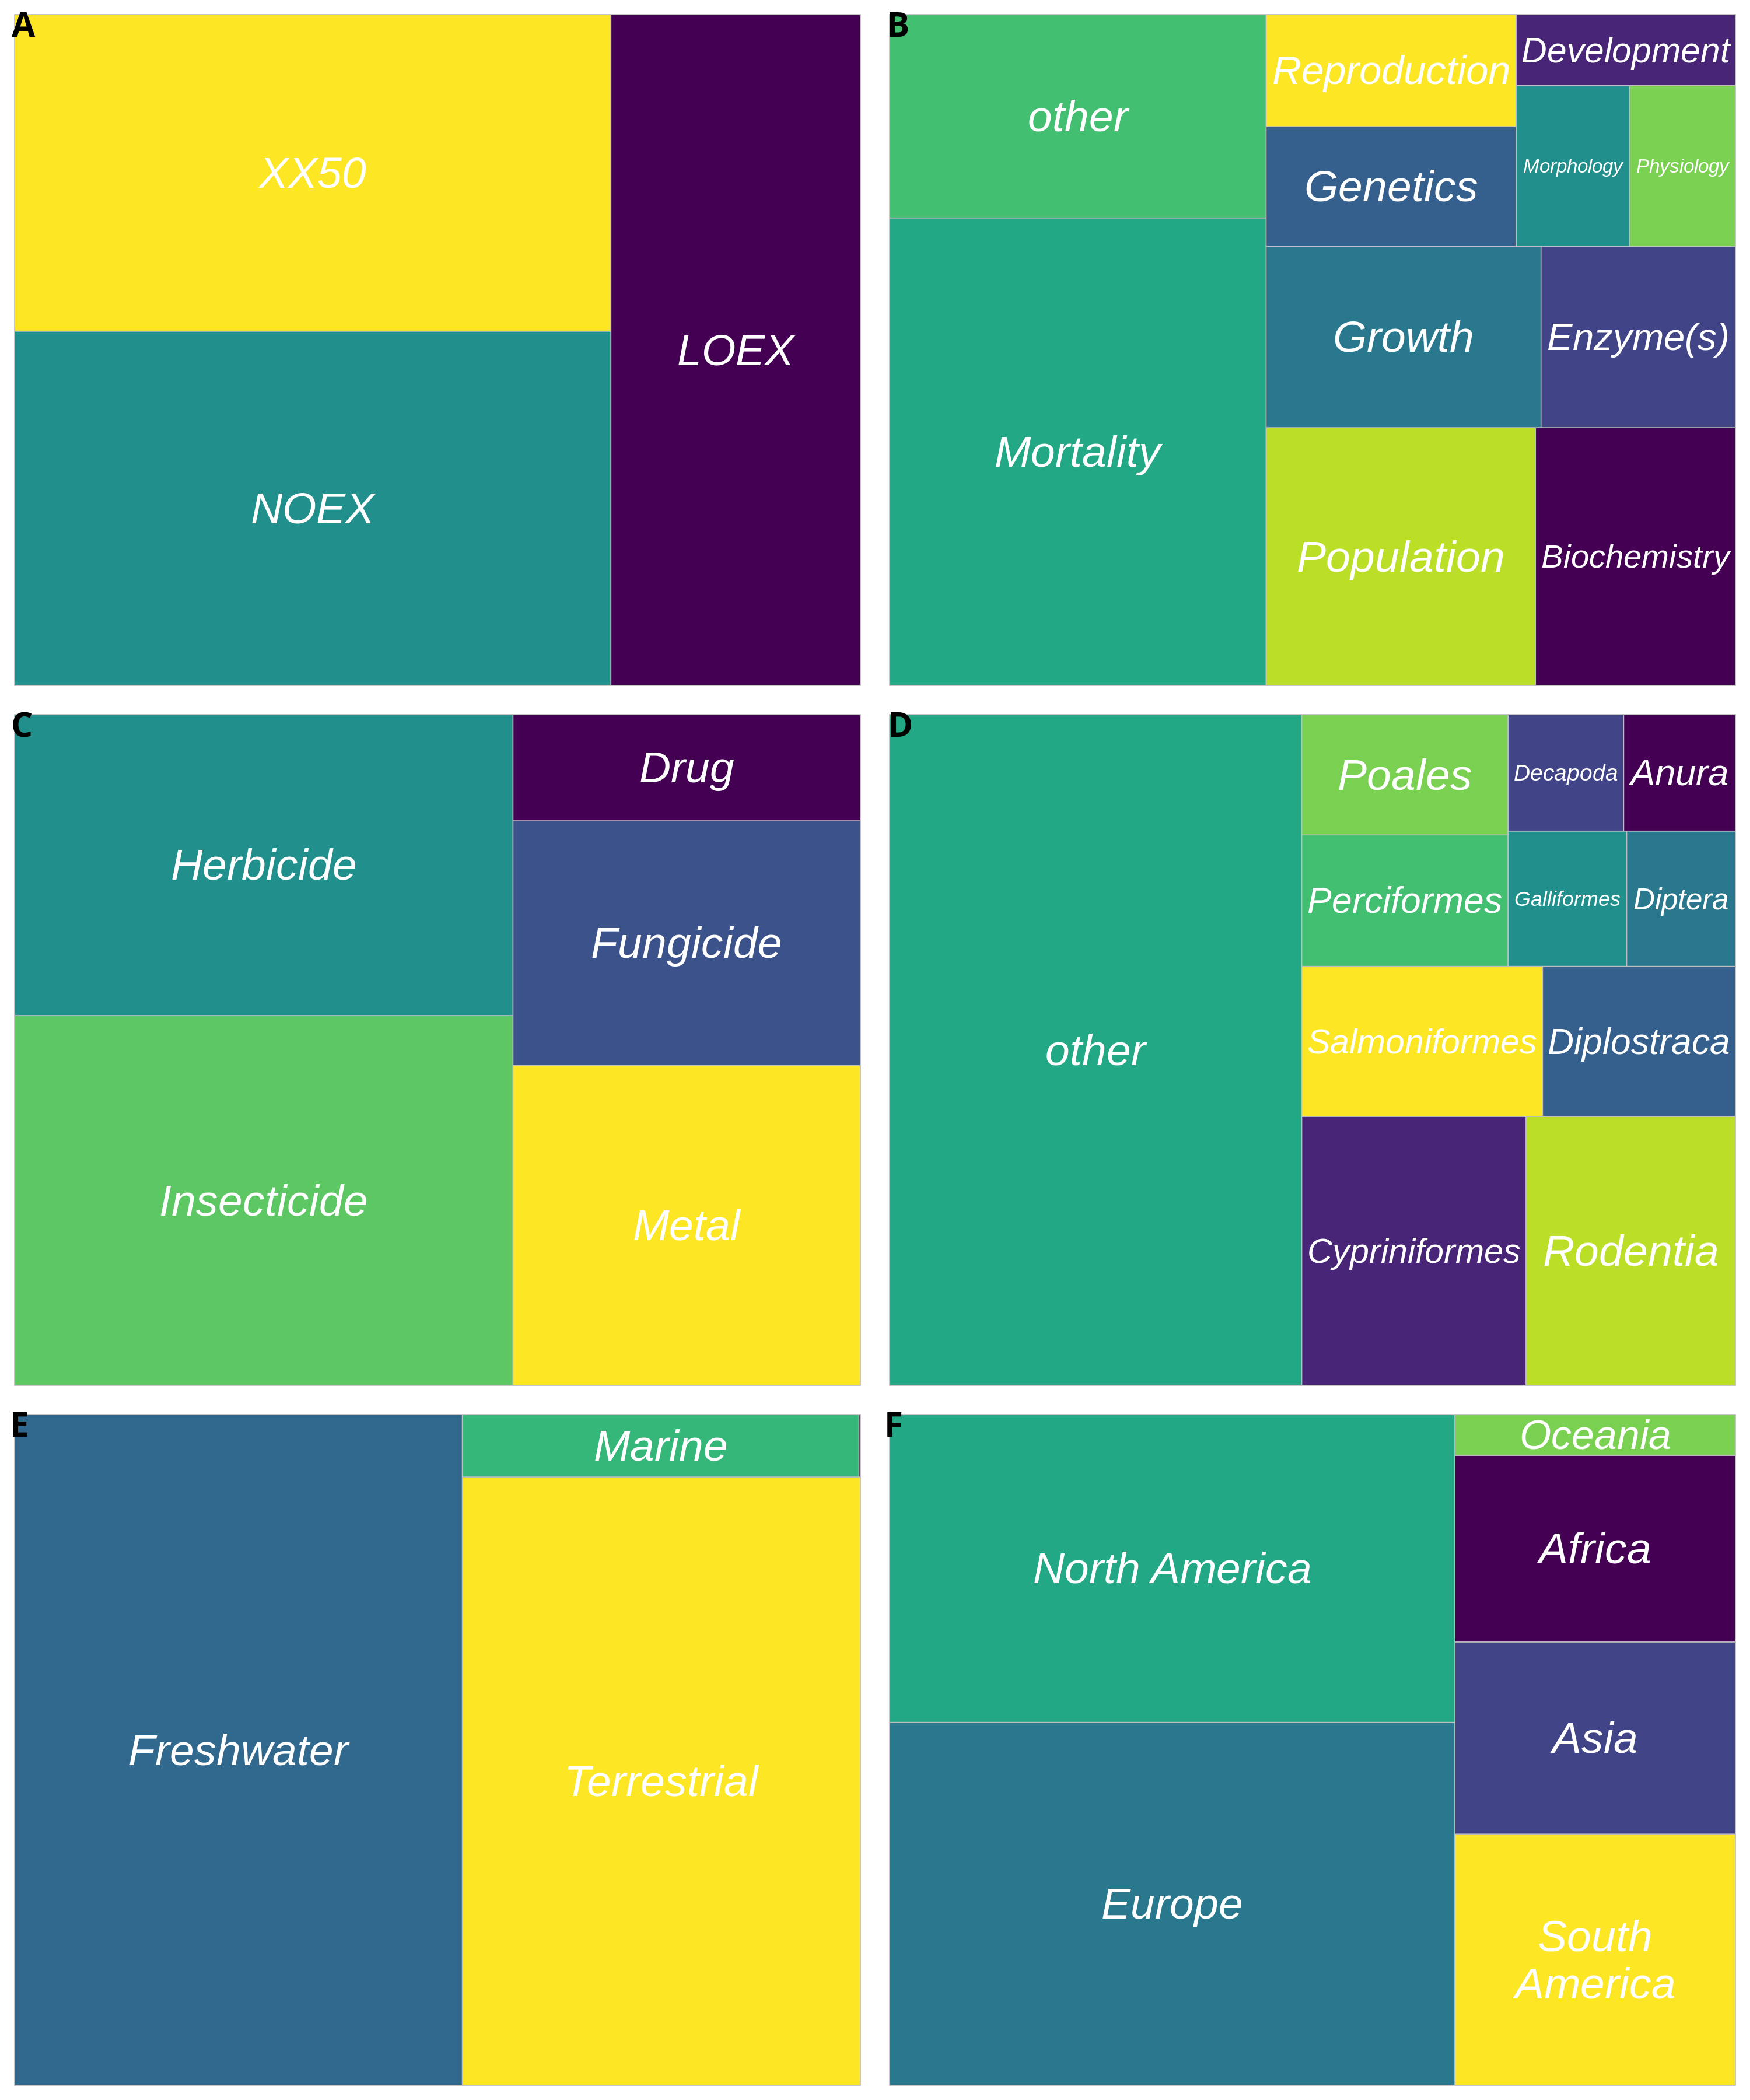
\includegraphics[width=0.8\textwidth]{article/figures/standartox_parameters.png}
    \caption{Share of 10 most frequent entries for the parameters (\textbf{A}) effect group, (\textbf{B}) chemical role, (\textbf{C}) chemical class, (\textbf{D}) taxonomic order, (\textbf{E}) organism habitat and (\textbf{F}) organism distribution in Standartox. Multiple classifications are possible (e.g. a chemical can be a fungicide and a pesticide).}
    \label{fig:stx-parameters}
\end{figure}

\subsection{Aggregation}
Typically, species exhibit a differential sensitivity towards chemicals (Figure~\ref{fig:stx-variability}A). Moreover, multiple ecotoxicity values are available for individual species-chemical combinations and these can also exhibit high variability due to several factors such as durations of ecotoxicity tests (Figure~\ref{fig:stx-variability}B), experimental conditions and physiological or genetic fitness differences between test individuals or populations. Not every factor is recorded though, leading to unexplainable variability (Figure~\ref{fig:stx-variability}C). To aggregate multiple ecotoxicity values into a single value on the desired taxonomic level (e.g. for an individual species, across species of a genus or family), and chemical grouping (e.g. across all pesticides), Standartox provides several aggregation methods including the minimum, the maximum and the geometric mean allowing to aggregate the filtered data set. The geometric mean is preferred in comparison to the arithmetic mean, because it is less influenced by outliers and is suitable for skewed data. Also, the geometric mean is preferable over the median, because the median completely ignores the tails of the data distribution, making it unreliable for small data sets \citep{leith_comparison_2010}. In the course of the aggregation process, outliers that exceed 1.5 times the interquartile range are flagged to caution Standartox users. However, they are considered in aggregation, given that the geometric mean is relatively robust against outliers. Overall, Standartox provides a harmonised and reproducible approach to data aggregation that may contribute to reduce between-study variability.

\begin{figure}[H]
    \centering
    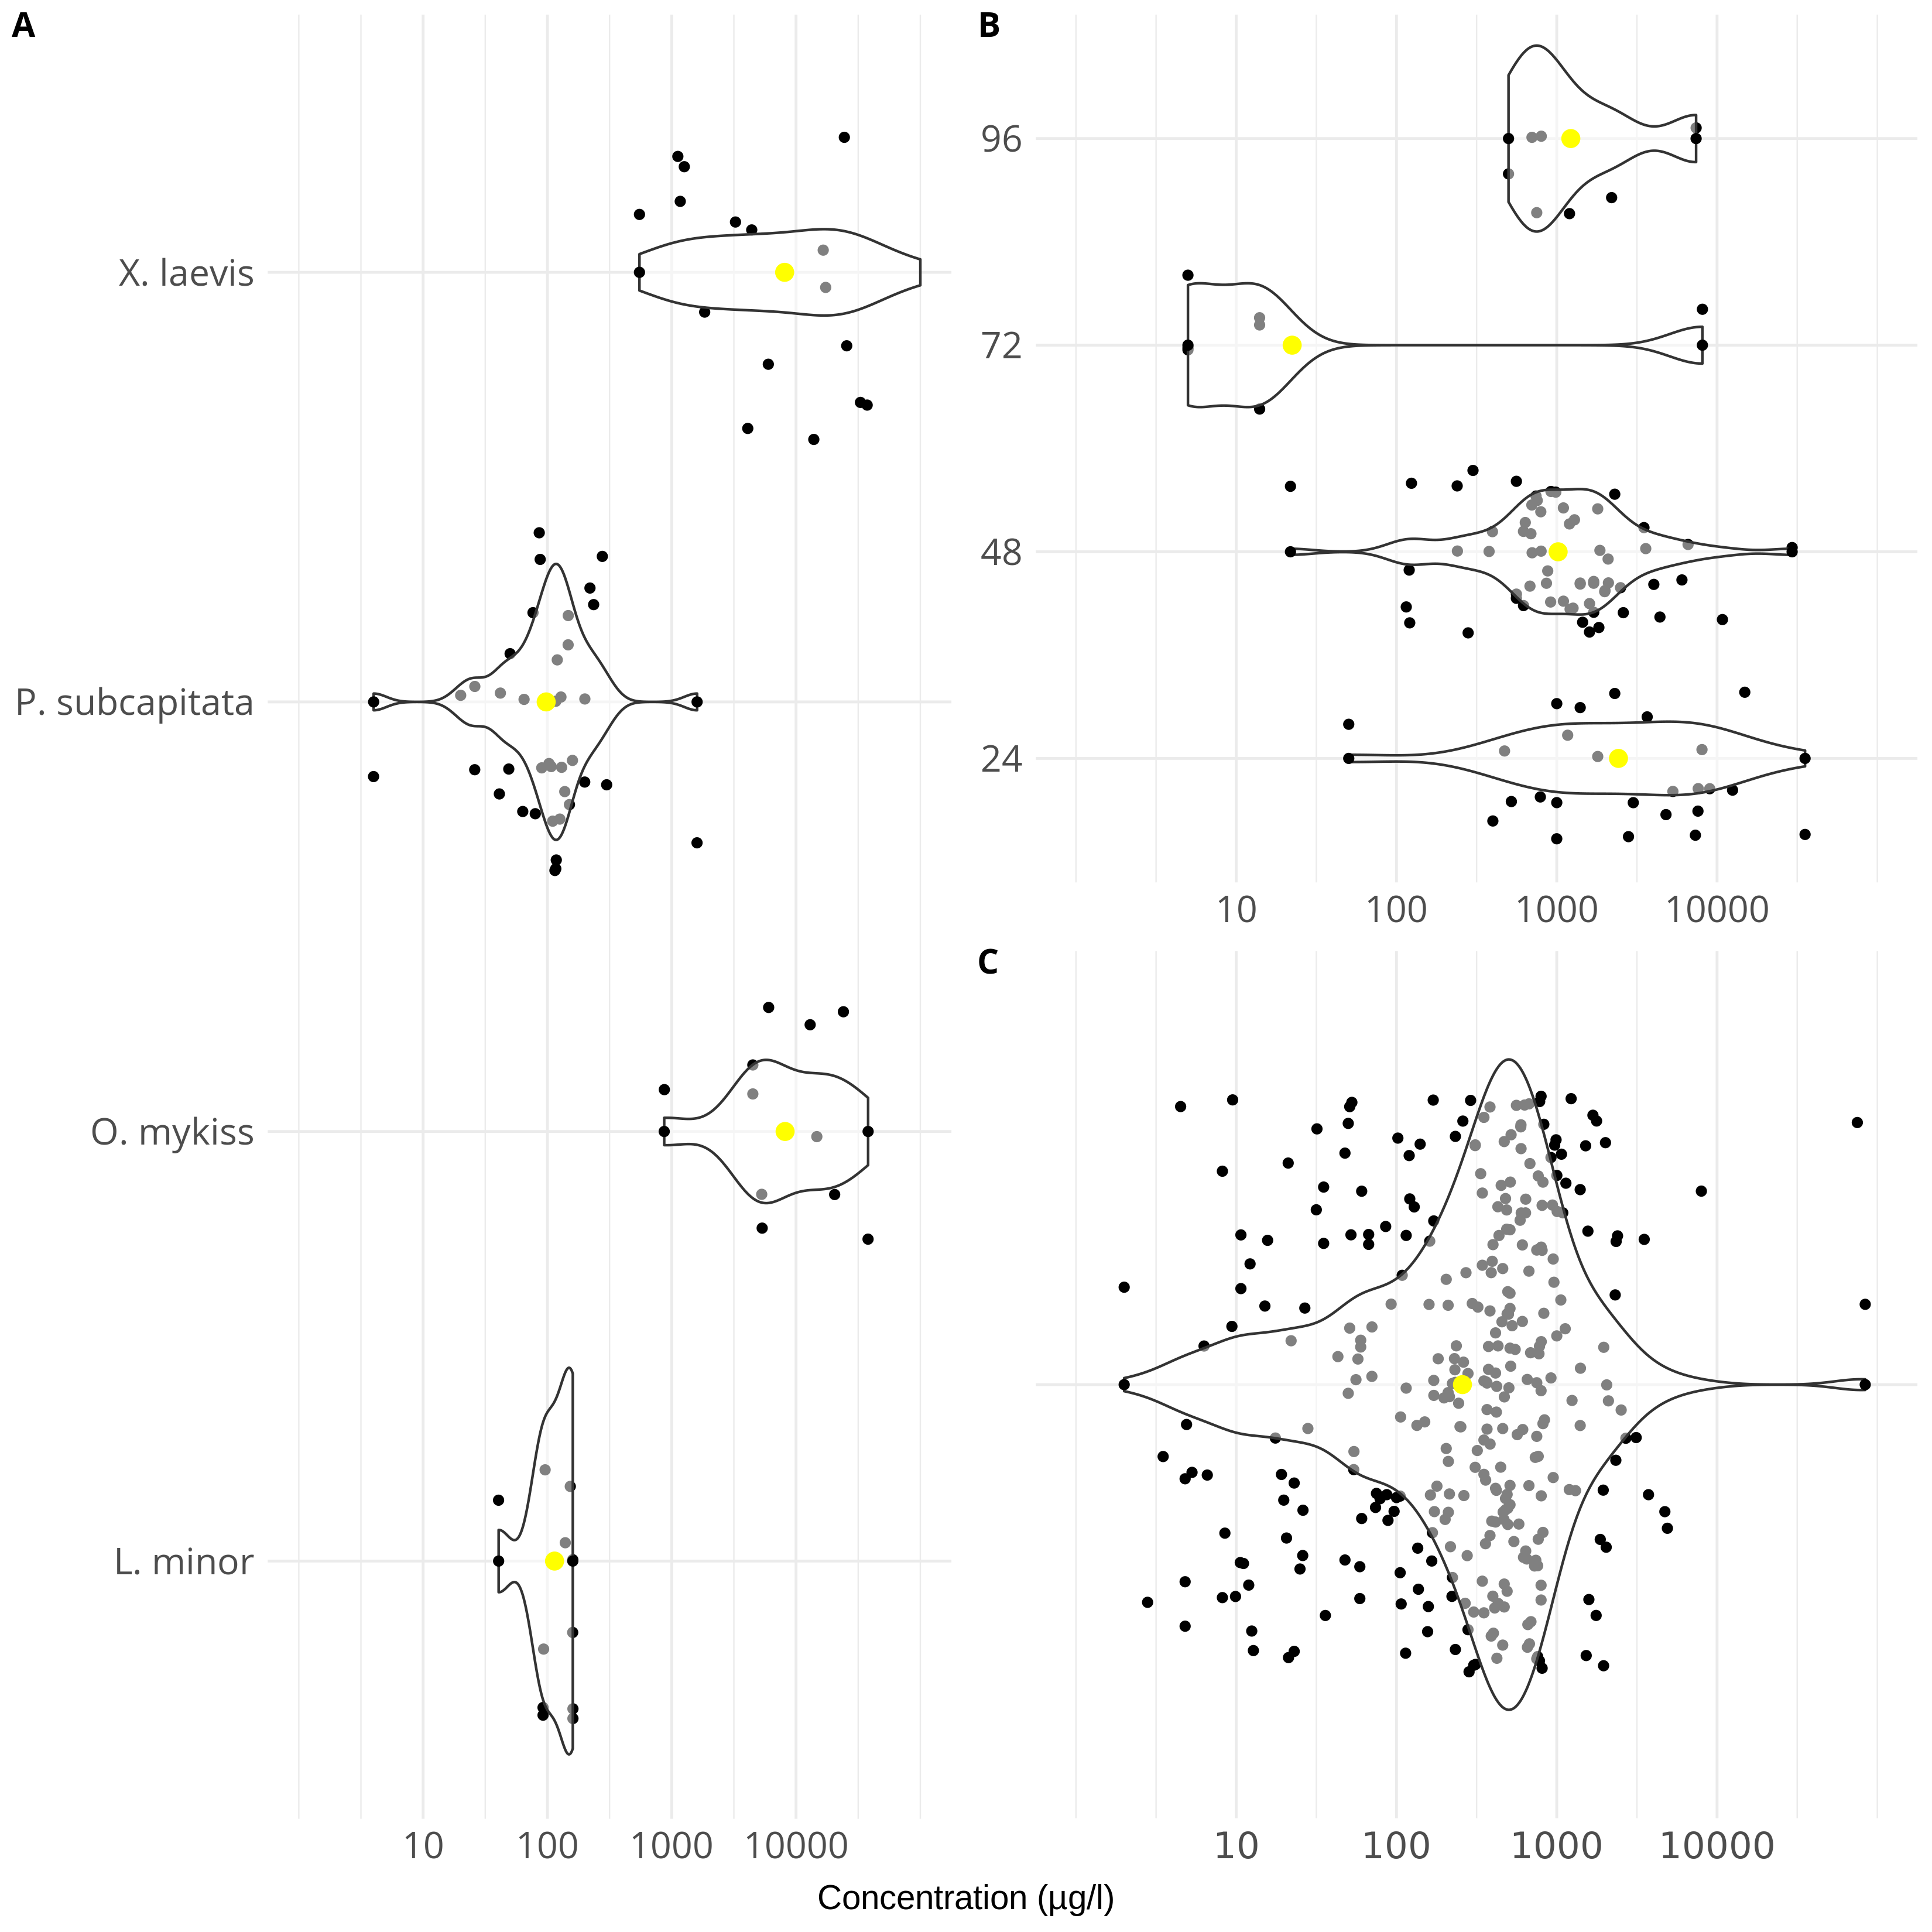
\includegraphics[width=0.8\textwidth]{article/figures/results_variability.png}
    \caption{Violin plots of of test results (EC\textsubscript{50}) in Standartox illustrating (\textbf{A}) differential variability and data distribution between species (i.e. \textit{Xenopus laevis} - Amphibia, \textit{Raphidocelis subcapitata} - Algae, \textit{Oncorhynchus mykiss} - fish, \textit{Lemna minor} - invertebrate) for the chemical atrazine in 96 h tests, (\textbf{B}) how the variability in toxicity tests with zinc sulfate and \textit{Daphnia magna} varies with test duration and (\textbf{C}) high variability that is not explained by the available test characteristics in the case of cupric sulfate tested on \textit{Pimephales promelas} for 96 h. Purple dots depict Standartox geometric mean estimates and black dots show raw data for each group. To facilitate readability, data points are randomly scattered along a hypothetical y-axis and are greyed out if within the violins.}
    \label{fig:stx-variability}
\end{figure}

\subsection{Accuracy Assessment}
To validate Standartox results we compared geometric means resulting from the aggregation in Standartox to the corresponding values from other databases, for chemicals where data was available in both resources. The PPDB provides ecotoxicity data on a few selected species from chemical risk assessment that have been manually quality controlled through expert judgement \citep{lewis_international_2016}. The vast majority of aggregated values (91~\%) of Standartox lie within one order of magnitude of the corresponding PPDB values (n = 3601). This would increase to 92.7~\%, when restricting the comparison to Standartox values where data from at least five experiments are available. Similarly, we compared Standartox to ecotoxicity values for \textit{D. magna} from the ChemProp \citep{ufzdepartmentofecologicalchemistry_chemprop_2019} software, which estimates LC\textsubscript{50} values via quantitative structure-activity relationship (QSAR) models \citep{schuurmann_quantitative_2011}. We found that 95~\% of Standartox values lie within one order of magnitude of the Chemprop (n = 179) values. However, the difference is not necessarily an indication of lower quality of Standartox estimates but may also reflect the wider range of experimental conditions for which data are available in the database underlying Standartox as well as inaccurate predictions for QSAR models, respectively (Figure~\ref{fig:standartox_ppdb_diff}).

\begin{figure}[H]
    \centering
    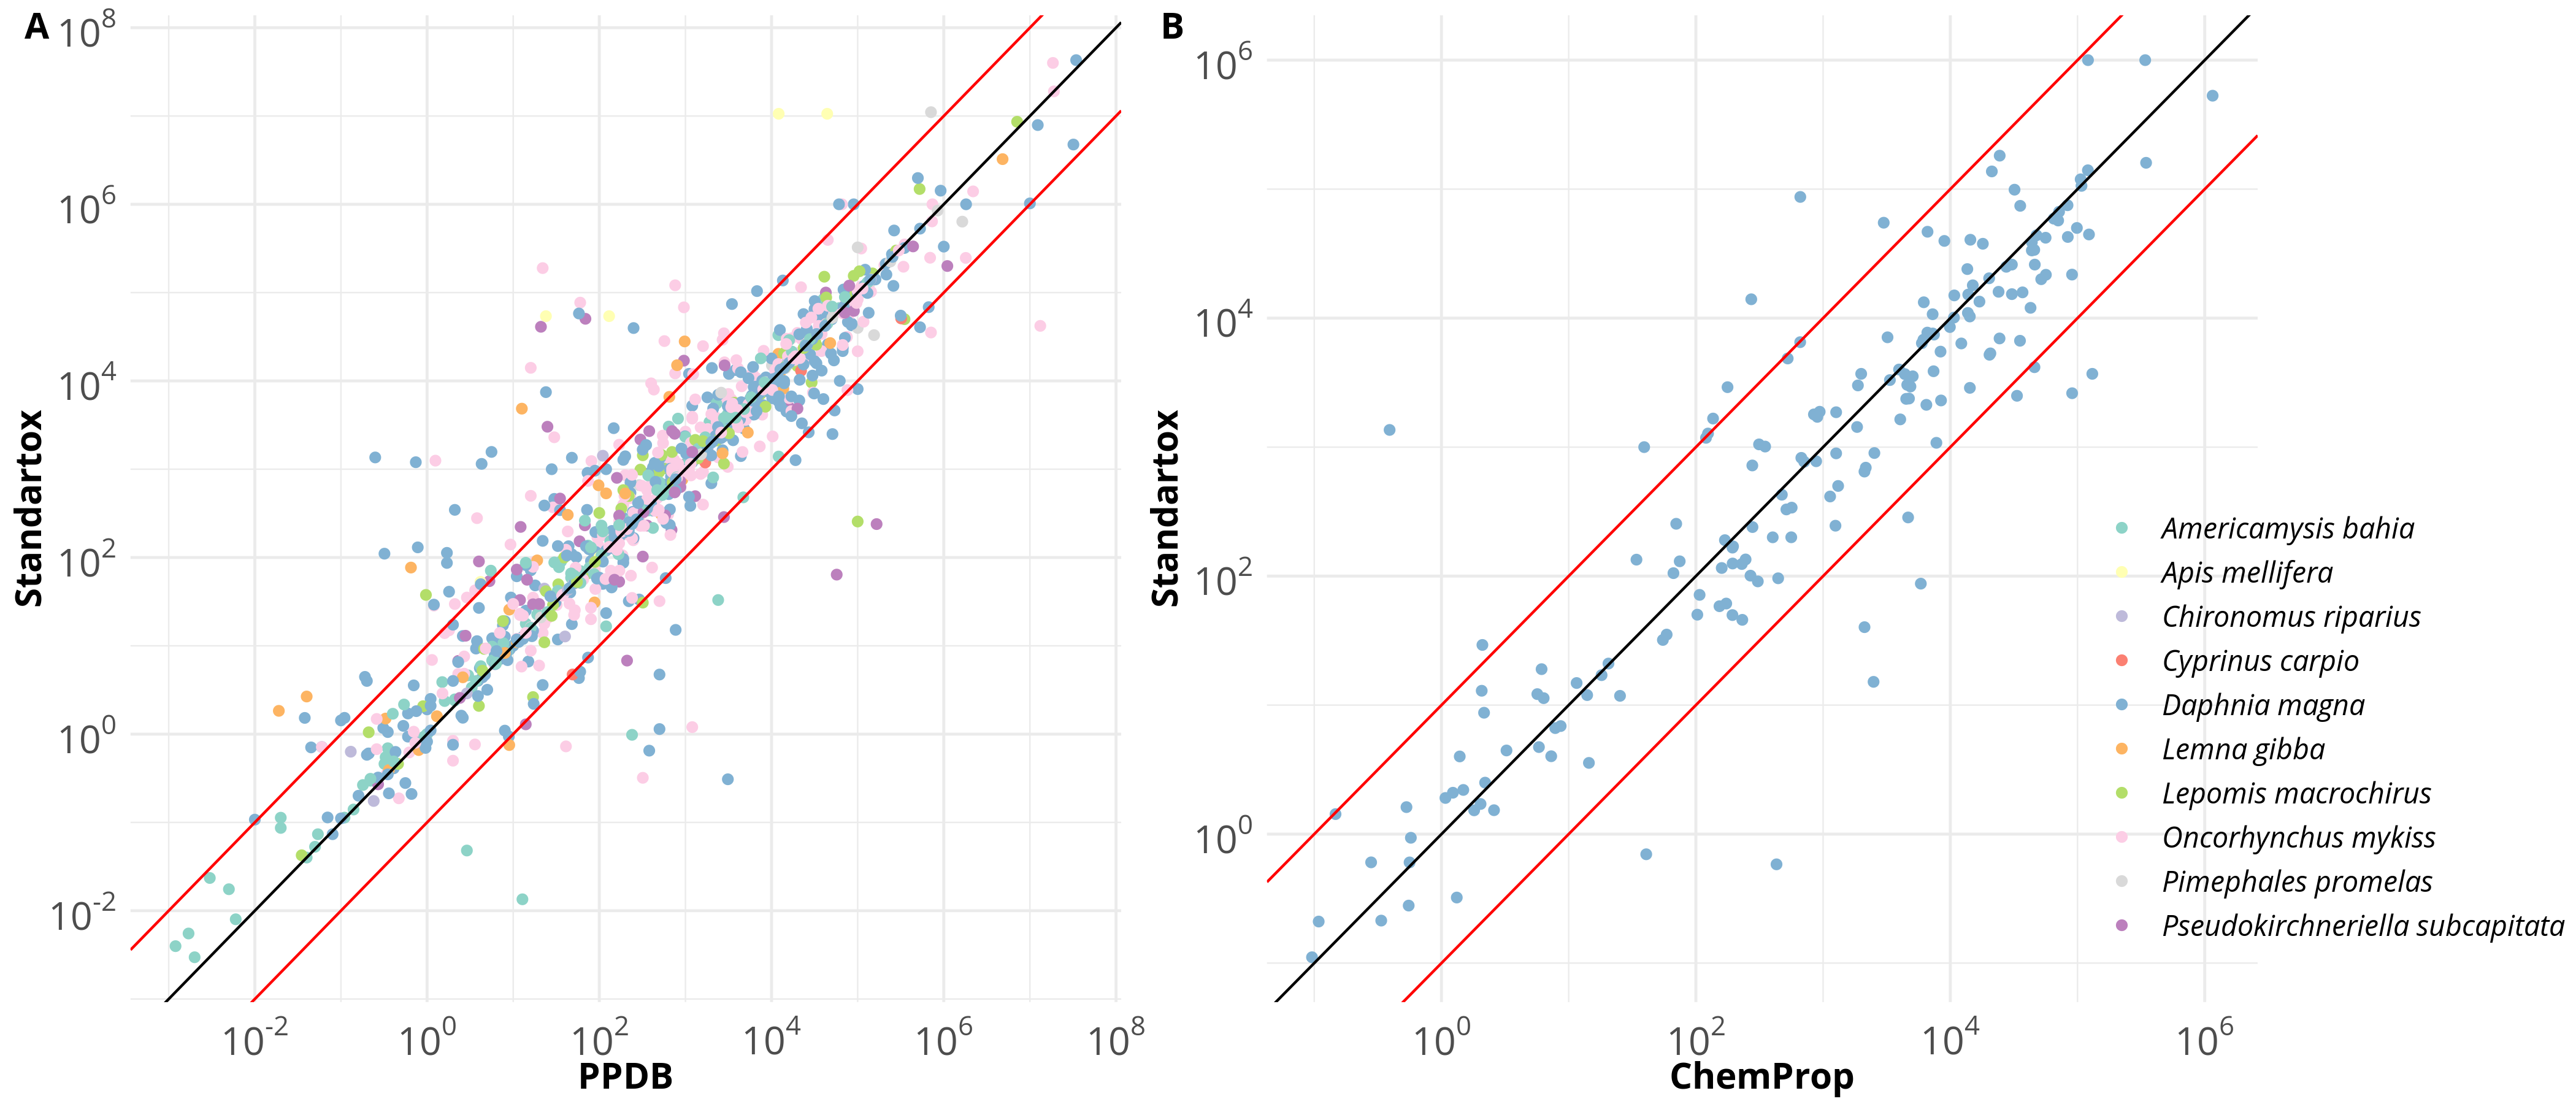
\includegraphics[width=1\linewidth]{article/figures/gg_ppdb_stan_compare_continous.png}
    \caption{Comparison between Standartox and (\textbf{A}) PPDB and (\textbf{B}) ChemProp values. The black lines indicate identity and red lines mark a divergence of a factor of 10. Compared species are color coded.}
    \label{fig:standartox_ppdb_diff}
\end{figure}

\subsection{Perspectives}
Novel predictive frameworks incorporating chemical mode of action and species traits emphasize the need for holistic and automated analyses of large-scale ecotoxicological data \citep{malaj_evolutionary_2016, vandenberg_modeling_2019}. Indeed, the increasing amount of data from ecotoxicological tests and experiments that is becoming available has elicited several initiatives to harmonize these data. These initiatives partly aim for overlapping goals, yet have limitations or objectives that distinguish them from Standartox:

\textbf{Comptox}, is a web tool published by the EPA which, similar to Standartox allows for filtering test results, the retrieval of additional chemical information and the estimation of toxicity data, such as 48 h \textit{Daphnia magna} LC\textsubscript{50} values. However, toxicity estimations are limited to standard test organisms (e.g. \textit{Daphnia magna}), and the tool lacks the possibility for automated retrieval \citep{williams_comptox_2017}.

The \textbf{EnviroTox} database which also uses, amongst others the ECOTOX database as an input has recently been published \citep{healthandenvironmentalsciencesinstitutehesi_envirotox_2019, connors_creation_2019}. In contrast to Standartox, EnviroTox  is restricted to selected aquatic organisms (i.e. fish, amphibians, invertebrates and algae) and experimental durations (at least 24 h) and uses a rule-based algorithm to derive single ecotoxicity values. Besides, EnviroTox provides additional information on toxicity endpoints, such as acute or chronic classifications and mode of action assignments. We intentionally omitted such classifications given that the approach to classification may vary with the purpose of the study. The EnviroTox database allows for an aggregation into single toxicity values for individual taxa, whereas Standartox performs this aggregation for individual taxa-chemical combinations. However, the Standartox results for individual taxa-chemical combinations could easily be aggregated across chemicals in a second step to provide a similar aggregation as that performed in EnviroTox.

The \textbf{Etox} database, like the ECOTOX database collects and provides filter methods for ecotoxicological test information.

The \textbf{PPDB} provides data only on pesticides and as mentioned before provides single quality controlled values only for commonly used taxa, e.g. \textit{D. magna} or \textit{R. subcapitata}.

\begin{table}[H]
    \caption{Overview on databases that provide ecotoxicological data. Abbreviations: \textbf{ALL:} Most important test parameters, including chemical, taxon, duration for filtering ecotoxicological data are incorporated. \textbf{WEB:} Accessible via a web application through a graphical user interface. \textbf{API:} Accessible via an application programming interface.}
    \label{tab:database-differences}
    \centering
    \begin{tabular}{m{3cm}m{3cm}m{2cm}m{2cm}m{1cm}}
    \toprule
    \textbf{Database} & \textbf{Publisher} & \textbf{Filter} & \textbf{Aggregation, Selection} & \textbf{Access} \\
    \midrule
    Comptox & Environmental Protection Agency & Chemical & no & WEB, file \\
    Ecotox & Environmental Protection Agency & ALL & no & WEB, file \\
    EnviroTox & Health and Environmental Sciences Institute & ALL & chemical, organism \\
    Etox & Umweltbundesamt & ALL & no & WEB \\
    Pesticides Properties DataBase (PPDB) & University of Hertfordshire & fixed values & manual selection & WEB, file \\
    Standartox & this article & ALL & chemical, organism & API, WEB \\
    \bottomrule
\end{tabular}
\end{table}

In summary, none of the above mentioned initiatives aim for an automated and standardized aggregation method of exposure endpoints for individual chemicals. In addition, they lack the possibility to access the databases through a common high level programming language, such as R. As outlined above, toxicity estimates from different studies can vary strongly due to a wide range of experimental conditions such as pH, temperature and conductivity \citep{rosenkrantz_influence_2013, li_temperature_2011}. Integrating these conditions into the aggregated estimates would certainly improve toxicity estimates. However, the current implementation of Standartox omits these conditions, because the ECOTOX database only provides sparse records on experimental conditions. The most frequently provided experimental conditions are temperature (77~\%), pH (56~\%), hardness (27~\%), dissolved oxygen (18~\%), Alkalinity (15~\%) and salinity (9~\%). For all other conditions less than 5~\% of data entries are available. A text-mining approach, where a literature reference is associated with ecotoxicity raw data, iterating through the individual publications could potentially increase this number. E.g. \citet{compson_linking_2018} successfully applied text-mining techniques to retrieve species trait data. 

%%%%%%%%%%%%%%%%%%%%%%%%%%%%%%%%%%%%%%%%%%
\section{Methods}
An automated processing pipeline downloads the quarterly released ECOTOX database, performs several preparation steps on it and exports a final Standartox data set. This data set is accessible via a web application and an application programming interface (API). An API provides the means for machine communication between a host and a client and thus allows scriptable data queries. To facilitate the API access, the R \citep{rcoreteam_language_2017} package \textit{standartox} is built. All data presented in this paper are derived from the Standartox build based on the ECOTOX release from the 12.12.2019. The code for Standartox is located in two Github repositories \url{https://github.com/andschar/standartox-build} and \url{https://github.com/andschar/standartox}. The former contains code to process the data and to build the web application and the API, the latter contains code to build the R-package. Most of the code is written in R 3.6.1 and associated packages (List: \ref{lis:r-packages}) and SQL for PostgreSQL 9.6.1.

\subsection{Processing}
Standartox downloads the quarterly released ECOTOX database and builds it into a local PostgreSQL database \citep{szocs_build_2019}. Subsequently, Structured Query Language (SQL) functions for further processing the data are implemented. In addition lookup tables that enable the conversion of units such as duration and concentration are created. A meta-table providing information such as the release version of the ECOTOX database is added. Then, provided Chemical Abstracts Service Numbers (CAS) and taxonomic names are used to query additional information from publicly available databases on chemicals and organisms, respectively. This includes the Compendium of Pesticide Common Names \citep{wood_compendium_2019}, the Chemical Entities of Biological Interest (ChEBI) database \citep{hastings_chebi_2016}, the Chemical Identifier Resolver (CIR) service \citep{nationalinstitutesofhealthnih_chemical_2019}, the Pubchem database \citep{kim_pubchem_2016}, Eurostat \citep{europeancommission_eurostat_2019} and Wikidata \citep{vrandecic_wikidata_2014} for chemicals and the World Register of Marine Species (WoRMS) \citep{wormseditorialboard_world_2018} and the Global Biodiversity Information Facility (GBIF) \citep{gbif_gbif_2019} (Table~\ref{tab:data-base-additional}) for habitat and spatial distribution of organisms. Given that CAS and taxonomic names can be ambiguous, e.g. the genus \textit{Eisenia} can refer to an algae and a worm, we first match them against the database specific identifiers and subsequently use them to retrieve the actual data. In a next step the data is added to Standartox to enable filtering for specific chemical roles (e.g. drug, metal, pesticide, personal care product) and classes (e.g. pyrethroid, carbamate) as well as spatial distribution (i.e. continents) and habitat preferences (e.g. freshwater) of individual taxa. Taxa that were not identified to at least genus level are excluded, because relative toxicity comparisons have been shown to be not meaningful for higher taxonomic levels \citep{rainbow_trace_2002, buchwalter_differences_2005, malaj_physiological_2012}. Finally, the Standartox data set is compiled, which includes the harmonisation of data, e.g. through conversion of test concentration and duration units. 1237 distinct concentration units are converted to X harmonised ones, as are the 126 distinct duration units to X. Standartox retains only duration units that can unambiguously be converted to hours. To guarantee appropriate unit conversion and harmonisation, we compared an automated to a manual conversion for each of the distinct concentration and duration units. Furthermore, the units are cleaned, for example through removing additional information in the field such as \textit{food}, \textit{soil}, \textit{ai} that are also coded in other variables and hinder the processing of units. Concentrations that are given as rates such as per day (e.g. mg/kg/day) are multiplied by the days of the test and then converted. Experimental endpoints are restricted to three groups, namely NOEX, LOEX and XX50. Other endpoints, such as Bioconcentration factors, non-half maximal effective concentrations (e.g. IC10, EC25, LD99) or maximum acceptable toxicant (MATC) concentrations are removed. Along with that, a catalog, listing all distinct entries and value ranges, for categorical and continuous variables, respectively, is created. Finally, we run quality control scripts that check the accuracy of the data. The compiled Standartox data set together with the catalog is exported and accessible via the web application and the API, through the R package.

\begin{figure}[H]
    \centering
    \includestandalone[scale=0.75]{article/tikz/standartox-organigram}
    \caption{Organigram of Standartox. The ECOTOX knowledge base is downloaded quarterly and processed (i.e. query additional information with CAS and taxa name and conversion of concentration and duration units. Subsequently, a Standartox data set is compiled together with filter and aggregation methods. Thus, users can access the Standartox data set and filter and aggregate through a web application and an R-package.}
    \label{fig:stx-organigram}
\end{figure}

\subsection{Application methods}
When accessed, the web application and the API load the compressed serialized Standartox data into memory and allow the user to interact with it. The user can then call the functions stx\_filter() and stx\_aggregate() that filter and aggregate the data according to specific parameters (Table~\ref{tab:app-parameters}). The interactive web application is built in R using the shiny framework, which runs with the help of a shiny server \citep{chang_shiny_2018} on \url{standartox.uni-landau.de}. The API is built by using the R package \textit{plumber} \citep{trestletechnologyllc_plumber_2018}, which allows for the creation of Representational State Transfer (REST) APIs from R. REST is a software architectural style that defines web service communication rules. The API is reachable via the URL \url{http://139.14.20.252} and port 8000. Four API-endpoints (\textit{/catalog}, \textit{/filter}, \textit{/aggregate} and \textit{/meta}) can be queried (Table~\ref{tab:api-endpoints}). The \textit{/catalog} API-endpoint returns a JavaScript Object Notation (JSON) file containing a catalog of possible filter parameters to choose from. The \textit{/filter} returns the filtered Standartox table as a compressed serialized binary file created by the R \textit{fst} package \citep{klik_fst_2019}, to reduce size and allow for fast user queries. The \textit{/aggregate} API-endpoint returns an R function allowing the client to aggregate the filtered data locally. Lastly, the \textit{/meta} API-endpoint returns a JSON file with meta information, such as the timestamp of the request and the used Standartox version. The API is designed to be used with the R-package \textit{standartox} and therefore uses serialization methods specific to R (rds() from the R package \textit{base} and fst() from the package \textit{fst}). To facilitate the API usage the R-package \textit{standartox} is created.

\begin{table}[H]
    \caption{Input parameters for the Standartox web application and the R-package standartox (CAS - Chemical Abstracts Service Registry Number, NOEX and XX50 - Standartox endpoints \ref{tab:endpoints-conflate}), vers - Standartox version).}
    \label{tab:app-parameters}
    \centering
    \begin{tabular}{cc}
    \toprule
    \textbf{parameter} & \textbf{example} \\ 
    \midrule
    cas & 7758987, 2921-88-2, 1912-24-9 \\
    concentration\_type & Active ingredient, Formulation \\
    chemical\_role & Antibiotic, Fungicide, Drug \\
    chemical\_class & Conazole, Neonicotinoid, Triazine \\
    taxa & Oncorhynchus mykiss, Rattus norvegicus, Daphnia magna \\
    habitat & Marine, Brackish, Freshwater \\
    region & Europe, Africa, Asia \\
    duration & 24, 96 \\
    effect & Mortality, Population, Growth \\
    endpoint & NOEX, XX50 \\
    exposure & auquatic, diet \\
    vers & 20191212 \\
    \bottomrule
\end{tabular}
\end{table}

%%%%%%%%%%%%%%%%%%%%%%%%%%%%%%%%%%%%%%%%%%
\section{User Notes - optional}
Users can access Standartox either via the web application \url{standartox.uni-landau.de} or via the R-package \textit{standartox}. By accessing the web application, users can filter and download the resulting data sets as a comma-separated values (csv) file. Users of the R-package can directly load the data within R. The R-package provides the two functions \textit{stx\_catalog()} and \textit{stx\_query()}. The first command queries a catalog of possible Standartox parameters into an R list object. The latter allows users to set the Standartox filter parameters and to fetch the actual data. It returns an R list of three tables (i.e. R data.frames) containing the filtered data set, the aggregated data set and a table with the meta information retrieved from the API endpoints. A short R-code example is given below (Listing \ref{lis:standartox-example}) and a detailed description on the usage of the R package is provided on its Github page: \url{https://github.com/andschar/standartox}.

\begin{lstlisting}[
    caption = {Sample code to access the Standartox data base through the API with the help of the R-package. \textit{stx\_catalog()} returns a catalog of possible filter and aggregation parameters. \textit{stx\_query()} returns the Standartox object, a list of the filtered and the aggregated data as well as a meta data entry.},
    label = {lis:standartox-example}]
    
# install
install.packages('remotes')
remotes::install_github('andschar/standartox') # package not yet on CRAN
# retrieve catalog    
require(standartox)
catal = stx_catalog()
# retrieve data
l = stx_query(cas = '1071-83-6',
                endpoint = 'XX50',
                taxa = 'Oncorhynchus',
                duration = c(24, 120))
\end{lstlisting}

%%%%%%%%%%%%%%%%%%%%%%%%%%%%%%%%%%%%%%%%%%
\section{Conclusion - optional}
% This section is not mandatory, but can be added to the manuscript if the discussion is unusually long or complex.
Due to the steady incorporation of new ecotoxicity data, the aggregated values produced by Standartox can be subject to change with future updates. We regard this as an advantage rather than a drawback because other published works that aim in a similar direction often constitute a singular effort or require manual work for each update. Standartox, in contrast automates the update process, yet still provides access to its older versions, assuring reproducability and version control. In comparison to rule-based approaches for the derivation of single ecotoxicity values, Standartox has the advantage to be free from the subjectivity of a set of human-induced rules. Above all, Standartox provides quick access through its design to be queried via the R language. Due to an increased amount of available ecotoxicological test data, it becomes fundamental to provide and distribute ecotoxicity information in adequate formats, both easily accessible for humans and easily processable for machines. Standartox meets these requirements and puts its focus on the aggregation of toxicity data, thereby adding a piece to the puzzle of modern ecotoxicological data analyses.


%%%%%%%%%%%%%%%%%%%%%%%%%%%%%%%%%%%%%%%%%%
\vspace{6pt} 

%%%%%%%%%%%%%%%%%%%%%%%%%%%%%%%%%%%%%%%%%%
%% optional
%\supplementary{The following are available online at \linksupplementary{s1}, Figure S1: title, Table S1: title, Video S1: title.}

% Only for the journal Methods and Protocols:
% If you wish to submit a video article, please do so with any other supplementary material.
% \supplementary{The following are available at \linksupplementary{s1}, Figure S1: title, Table S1: title, Video S1: title. A supporting video article is available at doi: link.}

%%%%%%%%%%%%%%%%%%%%%%%%%%%%%%%%%%%%%%%%%%
\authorcontributions{conceptualization and methods, A.S.,R.B.S. and V.C.S.; software development and validation, A.S.; data curation and analysis, A.S.; writing--original draft preparation, A.S.; writing--review and editing, A.S., V.C.S. and R.B.S.; supervision, R.B.S.}

%%%%%%%%%%%%%%%%%%%%%%%%%%%%%%%%%%%%%%%%%%
\funding{Please add: ``This research received no external funding'' or ``This research was funded by NAME OF FUNDER grant number XXX.'' and  and ``The APC was funded by XXX''. Check carefully that the details given are accurate and use the standard spelling of funding agency names at \url{https://search.crossref.org/funding}, any errors may affect your future funding.}

%%%%%%%%%%%%%%%%%%%%%%%%%%%%%%%%%%%%%%%%%%
\acknowledgments{In this section you can acknowledge any support given which is not covered by the author contribution or funding sections. This may include administrative and technical support, or donations in kind (e.g., materials used for experiments).}

%%%%%%%%%%%%%%%%%%%%%%%%%%%%%%%%%%%%%%%%%%
\conflictsofinterest{The authors declare no conflict of interest.} 

%%%%%%%%%%%%%%%%%%%%%%%%%%%%%%%%%%%%%%%%%%
\abbreviations{The following abbreviations are used in this manuscript:\\
\noindent 
\begin{tabular}{@{}ll}
API & Application programming interface \\
CAS & Chemical abstracts service registry Number \\
ChEBI & Chemical Entities of Biological Interest database \\
CIR & Chemical Identifier Resolver service \\
E/LC/D\textsubscript{50} &  Half maximal effective/lethal concentration/dose \\
ECOTOX & US EPA Ecotox Knowledgebase \\
GBIF & Global Biodiversity Information Facility \\
JSON & JavaScript Object Notation file format \\
LOEC/L & Lowest observed effect levels/concentration \\
NOEC/L & No observed effect levels/concentration \\
PPDB & Pesticides Properties DataBase \\
QSAR & Quantitative structure–activity relationship \\
REST & Representational state transfer software architectural style \\
SSD & Species sensitivity distribution \\
TU & Toxic unit \\
WoRMS & World Register of Marine Species \\
\end{tabular}
}

%%%%%%%%%%%%%%%%%%%%%%%%%%%%%%%%%%%%%%%%%%
%% optional
\appendixtitles{yes} %Leave argument "no" if all appendix headings stay EMPTY (then no dot is printed after "Appendix A"). If the appendix sections contain a heading then change the argument to "yes".
\appendix
\section{}
\begin{table}[H]
    \caption{Table of additionally queried publicly available data bases and their URLs.}
    \label{tab:data-base-additional}
    \centering
\begin{tabular}{cc}
    \toprule
    \textbf{Data Base} & \textbf{URL} \\ 
    \midrule
    \makecell{Chemical Entities of \\ Biological Interest (ChEBI)} & \url{https://www.ebi.ac.uk/chebi}  \\
    Chemical Identifier Resolver & \url{https://cactus.nci.nih.gov/chemical/structure}  \\[0.5cm]
    ChemSpider & \url{http://www.chemspider.com}    \\[0.5cm]
    Eurostat & \url{https://ec.europa.eu/eurostat/home} \\[0.5cm]
    PubChem & \url{https://pubchem.ncbi.nlm.nih.gov} \\[0.5cm]
    Wikidata & \url{https://www.wikidata.org/wiki/Wikidata:Main_Page} \\[0.5cm]
    \makecell{Global Biodiversity \\ Information Facility (GBIF)} & \url{https://www.gbif.org} \\[0.5cm]
    \makecell{World Register of \\ Marine Species (WoRMS)} & \url{http://marinespecies.org} \\
    \bottomrule
\end{tabular}
\end{table}

\begin{table}[H]
    \caption{Table of how Standartox endpoints are derived from EPA ECOTOX endpoints.}
    \label{tab:endpoints-conflate}
    \centering
\begin{tabular}{ccc}
    \toprule
    \textbf{Standartox endpoint} & \textbf{Ecotox endpoint} & \textbf{Ecotox endpoint description} \\
    \midrule
    XX50 & LC50 & Lethal concentration to 50\% of test organisms \\
    XX50 & LD50 & Lethal dose to 50\% of test organisms \\
    XX50 & EC50 & Effective concentration to 50\% of test organisms \\
    XX50 & ED50 & Effective dose to 50\% of test organisms \\
    XX50 & IC50 & Inhibition concentration to 50\% of test organisms \\
    XX50 & ID50 & Inhibition dose to 50\% of test organisms \\
    XX50 & ET50 & Effective response time to 50\% of test organisms \\
    XX50 & LT50 & Time to 50\% mortality of test organisms \\
    NOEX & NOEC & No-observable-effect-concentration \\
    NOEX & NOEL & No-observable-effect-level \\
    LOEX & LOEC & Lowest observable effect concentration\\
    LOEX & LOEL & Lowest-observable-effect-level \\
    \bottomrule
\end{tabular}
\end{table}

\begin{table}[H]
    \caption{Application programming interface (API) endpoints, Http methods, Requests and Response objects. JSON - Javascript opject notation file}
    \label{tab:api-endpoints}
    \centering
\begin{tabular}{cccc}
    \toprule
    \textbf{Endpoint} & \textbf{Http Method} & \textbf{Request} & \textbf{Response} \\
    \midrule
    /catalog & POST & Standartox version string & Catalog object (JSON) \\
    /filter & POST & Standartox filter parameters & Filtered Standartox data (serialized) \\
    /aggregate & GET & / & Aggregate function (serialized) \\
    /meta & POST & Standartox version string & Meta data on request (JSON) \\
    \bottomrule
\end{tabular}
\end{table}

\section{}

\begin{table}[H]
    \caption{R-packages used for the compilation of the Standartox database.}
    \label{tab:rpackages}
    \centering
\begin{tabular}{ccc}
\toprule
\textbf{Package} & \textbf{Description} & \textbf{Citation} \\ 
\midrule
bib2df & Parse a BibTeX File to a Data Frame & \citep{R-bib2df} \\
countrycode & Convert Country Names and Country Codes & \citep{R-countrycode} \\
cowplot & Streamlined Plot Theme and Plot Annotations for 'ggplot2' & \citep{R-cowplot} \\
data.table & Extension of `data.frame` & \citep{R-data.table} \\
DBI & R Database Interface & \citep{R-DBI} \\
dbreport & Automated reports from tables & \citep{R-dbreport} \\
devtools & Tools to Make Developing R Packages Easier & \citep{R-devtools} \\
doParallel & Foreach Parallel Adaptor for the 'parallel' Package & \citep{R-doParallel} \\
DT & A Wrapper of the JavaScript Library 'DataTables' & \citep{R-DT} \\
foreach & Provides Foreach Looping Construct for R & \citep{R-foreach} \\
fst & Lightning Fast Serialization of Data Frames for R & \citep{R-fst} \\
ggplot2 & Create Elegant Data Visualisations Using the Grammar of Graphics & \citep{R-ggplot2} \\ httr & Tools for Working with URLs and HTTP & \citep{R-httr} \\
jsonlite & A Robust, High Performance JSON Parser and Generator for R & \citep{R-jsonlite} \\
knitr & A General-Purpose Package for Dynamic Report Generation in R & \citep{R-knitr} \\
openxlsx & Read, Write and Edit xlsx Files & \citep{R-openxlsx} \\
plotly & Create Interactive Web Graphics via 'plotly.js' & \citep{R-plotly} \\
plumber & An API Generator for R & \citep{R-plumber} \\
R.utils & Various Programming Utilities & \citep{R-R.utils} \\
RColorBrewer & ColorBrewer Palettes & \citep{R-RColorBrewer} \\
reactlog & Reactivity Visualizer for 'shiny' & \citep{R-reactlog} \\
readxl & Read Excel Files & \citep{R-readxl} \\
rgbif & Interface to the Global 'Biodiversity' Information Facility API & \citep{R-rgbif} \\ RPostgreSQL & R Interface to the 'PostgreSQL' Database System & \citep{R-RPostgreSQL} \\
rvest & Easily Harvest (Scrape) Web Pages & \citep{R-rvest} \\
scales & Scale Functions for Visualization & \citep{R-scales} \\
shiny & Web Application Framework for R & \citep{R-shiny} \\
shinydashboard & Create Dashboards with 'Shiny' & \citep{R-shinydashboard} \\
shinydashboardPlus & Add More 'AdminLTE2' Components to 'shinydashboard' & \citep{R-shinydashboardPlus} \\
shinyjs & Easily Improve the User Experience of Your Shiny Apps in Seconds & \citep{R-shinyjs} \\ shinyWidgets & Custom Inputs Widgets for Shiny & \citep{R-shinyWidgets} \\
stringi & Character String Processing Facilities & \citep{R-stringi} \\
stringr & Simple, Consistent Wrappers for Common String Operations & \citep{R-stringr} \\
taxize & Taxonomic Information from Around the Web & \citep{R-taxize} \\
treemap & Treemap Visualization & \citep{R-treemap} \\
treemapify & Draw Treemaps in 'ggplot2' & \citep{R-treemapify} \\
udunits2 & Udunits-2 Bindings for R & \citep{R-udunits2} \\
webchem & Chemical Information from the Web & \citep{R-webchem} \\
\bottomrule
\end{tabular}
\end{table}

% \unskip
% \subsection{}
% The appendix is an optional section that can contain details and data supplemental to the main text. For example, explanations of experimental details that would disrupt the flow of the main text, but nonetheless remain crucial to understanding and reproducing the research shown; figures of replicates for experiments of which representative data is shown in the main text can be added here if brief, or as Supplementary data. Mathematical proofs of results not central to the paper can be added as an appendix.

% \section{}
% All appendix sections must be cited in the main text. In the appendixes, Figures, Tables, etc. should be labeled starting with `A', e.g., Figure A1, Figure A2, etc. 



%%%%%%%%%%%%%%%%%%%%%%%%%%%%%%%%%%%%%%%%%%
% Citations and References in Supplementary files are permitted provided that they also appear in the reference list here. 

%=====================================
% References, variant A: internal bibliography
%=====================================
% \begin{thebibliography}{999}
% Reference 1
% \bibitem[Author1(year)]{ref-journal}
% Author1, T. The title of the cited article. {\em Journal Abbreviation} {\bf 2008}, {\em 10}, 142--149.
% Reference 2
% \bibitem[Author2(year)]{ref-book}
% Author2, L. The title of the cited contribution. In {\em The Book Title}; Editor1, F., Editor2, A., Eds.; Publishing House: City, Country, 2007; pp. 32--58.
% \end{thebibliography}

% The following MDPI journals use author-date citation: Arts, Econometrics, Economies, Genealogy, Humanities, IJFS, JRFM, Laws, Religions, Risks, Social Sciences. For those journals, please follow the formatting guidelines on http://www.mdpi.com/authors/references
% To cite two works by the same author: \citeauthor{ref-journal-1a} (\citeyear{ref-journal-1a}, \citeyear{ref-journal-1b}). This produces: Whittaker (1967, 1975)
% To cite two works by the same author with specific pages: \citeauthor{ref-journal-3a} (\citeyear{ref-journal-3a}, p. 328; \citeyear{ref-journal-3b}, p.475). This produces: Wong (1999, p. 328; 2000, p. 475)

%=====================================
% References, variant B: external bibliography
%=====================================
\reftitle{References}
\nocite{*}
\externalbibliography{yes}
\bibliography{refs/references-standartox.bib,
              refs/references-standartox-rpackages.bib}

%%%%%%%%%%%%%%%%%%%%%%%%%%%%%%%%%%%%%%%%%%
%% optional
% \sampleavailability{Samples of the compounds ...... are available from the authors.}

%% for journal Sci
%\reviewreports{\\
%Reviewer 1 comments and authors’ response\\
%Reviewer 2 comments and authors’ response\\
%Reviewer 3 comments and authors’ response
%}

%%%%%%%%%%%%%%%%%%%%%%%%%%%%%%%%%%%%%%%%%%
\end{document}

